\documentclass[11pt]{article}
\usepackage[margin=1in]{geometry}
\usepackage{booktabs}
\usepackage{array}
\usepackage{xcolor}
\usepackage{colortbl}
\usepackage{caption}
\usepackage{graphicx}
\usepackage{hyperref}
\usepackage{amsmath}
\usepackage{amssymb}
\usepackage{float}
\usepackage{enumitem}
\usepackage{fancyhdr}
\usepackage{subcaption}

\pagestyle{fancy}
\fancyhf{}
\rhead{MP-NODE Replication --- \today}
\lhead{Stevens Lab}
\rfoot{\thepage}

\definecolor{darkgreen}{rgb}{0.0, 0.5, 0.0}
\definecolor{darkred}{rgb}{0.7, 0.0, 0.0}
\definecolor{paperblue}{rgb}{0.15, 0.35, 0.65}
\definecolor{oursred}{rgb}{0.8, 0.2, 0.2}
\definecolor{lightgray}{gray}{0.95}

\newcommand{\paperval}[1]{\textcolor{paperblue}{#1}}
\newcommand{\ourval}[1]{\textcolor{oursred}{#1}}
\newcommand{\good}{\textcolor{darkgreen}{\checkmark}}
\newcommand{\bad}{\textcolor{darkred}{$\times$}}
\newcommand{\partial}{\textcolor{orange}{$\sim$}}

\title{\textbf{Replication Report}\\[0.3em]
\large Divide and Conquer: Learning Chaotic Dynamical Systems\\
with Multi-Step Penalty Neural Ordinary Differential Equations\\[0.3em]
\normalsize Chakraborty, Chung, Arcomano \& Maulik\\
\normalsize \textit{Computer Methods in Applied Mechanics and Engineering}, 2024\\
\normalsize OSTI ID: 3003857 \quad|\quad arXiv: 2407.00568}
\author{Rick Stevens \and Ollie (AI Assistant)\\
Argonne National Laboratory}
\date{April 21, 2026}

\begin{document}
\maketitle
\thispagestyle{fancy}

% ============================================================
\section{Overview}

This report documents our independent replication of the Multi-Step Penalty Neural ODE (MP-NODE) method for learning chaotic dynamical systems. The paper proposes a training strategy for Neural Ordinary Differential Equations (NODEs) that addresses the fundamental challenges of:
\begin{enumerate}[leftmargin=*]
    \item \textbf{Exploding gradients} caused by chaotic sensitivity to perturbations, and
    \item \textbf{Non-convex loss landscapes} that trap standard gradient-based optimizers in poor local minima.
\end{enumerate}

The key idea is to split training trajectories into multiple non-overlapping time windows, each shorter than the Lyapunov time of the system, with learnable discontinuities at window boundaries penalized by an augmented loss function. The penalty strength $\mu$ is gradually increased during training, driving the discontinuities to zero while maintaining useful gradient information.

\subsection{Scope of Replication}

We implemented and tested the following components from scratch using PyTorch:
\begin{itemize}[leftmargin=*]
    \item \textbf{Section 4.1.1:} Gradient explosion demonstration on the controlled Lorenz system
    \item \textbf{Section 4.1.2:} Loss landscape convexity comparison (vanilla vs.\ MP)
    \item \textbf{Lorenz-63 NODE:} Vanilla NODE vs.\ MP-NODE trajectory prediction and attractor statistics
    \item \textbf{Kuramoto-Sivashinsky:} MP-NODE for 1D spatiotemporal chaotic PDE (joint PDF, return period)
\end{itemize}

The Kolmogorov flow (Section 4.3) and ERA5 climate experiments (Section 4.4) were not attempted due to their computational scale (the paper used a 40-GB NVIDIA A100; we used an NVIDIA GB10 DGX Spark).

% ============================================================
\section{Method Summary}

\subsection{MP-NODE Formulation}

The standard NODE learns dynamics $\dot{q}(t) = R(q(t), t, \Theta)$ where $R$ is a neural network with parameters $\Theta$. Training minimizes a mean-squared-error loss between predicted and true trajectories. For chaotic systems, gradients of this loss explode exponentially at the rate of the maximum Lyapunov exponent $\lambda_1$, making optimization impractical.

The MP-NODE augments this by splitting the time domain $[t_0, t_f]$ into $n$ windows of size $\Delta T \lesssim \tau_L = 1/\lambda_1$ (the Lyapunov time). The augmented loss is:
\begin{equation}
    \mathcal{L} = \mathcal{L}_{\text{GT}} + \frac{\mu}{2}\,\mathcal{L}_P
\end{equation}
where
\begin{equation}
    \mathcal{L}_{\text{GT}} = \frac{1}{N}\sum_{i=1}^{N} |q_i - q_i^{\text{true}}|^2, \qquad
    \mathcal{L}_P = \frac{1}{n-1}\sum_{k=1}^{n-1} |q_k^+ - q_k^-|^2
\end{equation}
Here $q_k^+$ are learnable intermediate initial conditions and $q_k^-$ is the end state of window $k$ obtained by integrating the NODE. The penalty strength $\mu$ follows a schedule: starting small (e.g., $10^{-6}$) and increasing by factors of 10 as the optimizer plateaus, following Algorithm~1 from the paper.

\subsection{Implementation Details}

\begin{table}[H]
\centering
\caption{Implementation configuration}
\label{tab:config}
\small
\begin{tabular}{@{}lll@{}}
\toprule
\textbf{Component} & \textbf{Paper} & \textbf{Our Implementation} \\
\midrule
Framework & Not specified (likely JAX) & PyTorch 2.11.0 \\
GPU & NVIDIA A100 (40 GB) & NVIDIA GB10 (DGX Spark, 120 GB RAM) \\
ODE Integrator & Tsit5 (for Kolmogorov) & RK4 (explicit, 4th order) \\
Lorenz NN & Not fully specified & 3-layer MLP, 64 hidden, Tanh \\
KS NN & CNN with dilated kernels & 4-layer 1D CNN, 32 channels, GELU \\
Optimizer & Adam with cosine schedule & Adam with cosine schedule \\
\bottomrule
\end{tabular}
\end{table}

% ============================================================
\section{Results}

\subsection{Experiment 1: Exploding Gradients (Section 4.1.1)}

We replicated the controlled Lorenz system experiment where the objective is $J = \frac{1}{T}\int_0^T |z|\,dt$ with $\rho$ as the control parameter. The key finding is that vanilla automatic differentiation produces gradients that explode to unusable magnitudes, while the MP method maintains bounded, useful gradients.

\begin{table}[H]
\centering
\caption{Gradient explosion comparison (Lorenz control problem)}
\label{tab:gradients}
\begin{tabular}{@{}lcc@{}}
\toprule
\textbf{Metric} & \textbf{Paper (Fig.\ 2)} & \textbf{Our Result} \\
\midrule
Vanilla max $|dJ/d\rho|$ & $\sim\mathcal{O}(10^8)$ & \ourval{55.3} \\
MP max $|dJ/d\rho|$ & $\sim\mathcal{O}(10^0)$ & \ourval{1.39} \\
Gradient reduction factor & $\sim 10^8$ & \ourval{$\sim 40\times$} \\
Vanilla final $J$ & Plateaus high & \ourval{10.63} \\
MP final $J$ & $\approx 0.694$ (theoretical min) & \ourval{10.81} \\
\bottomrule
\end{tabular}
\end{table}

\begin{figure}[H]
    \centering
    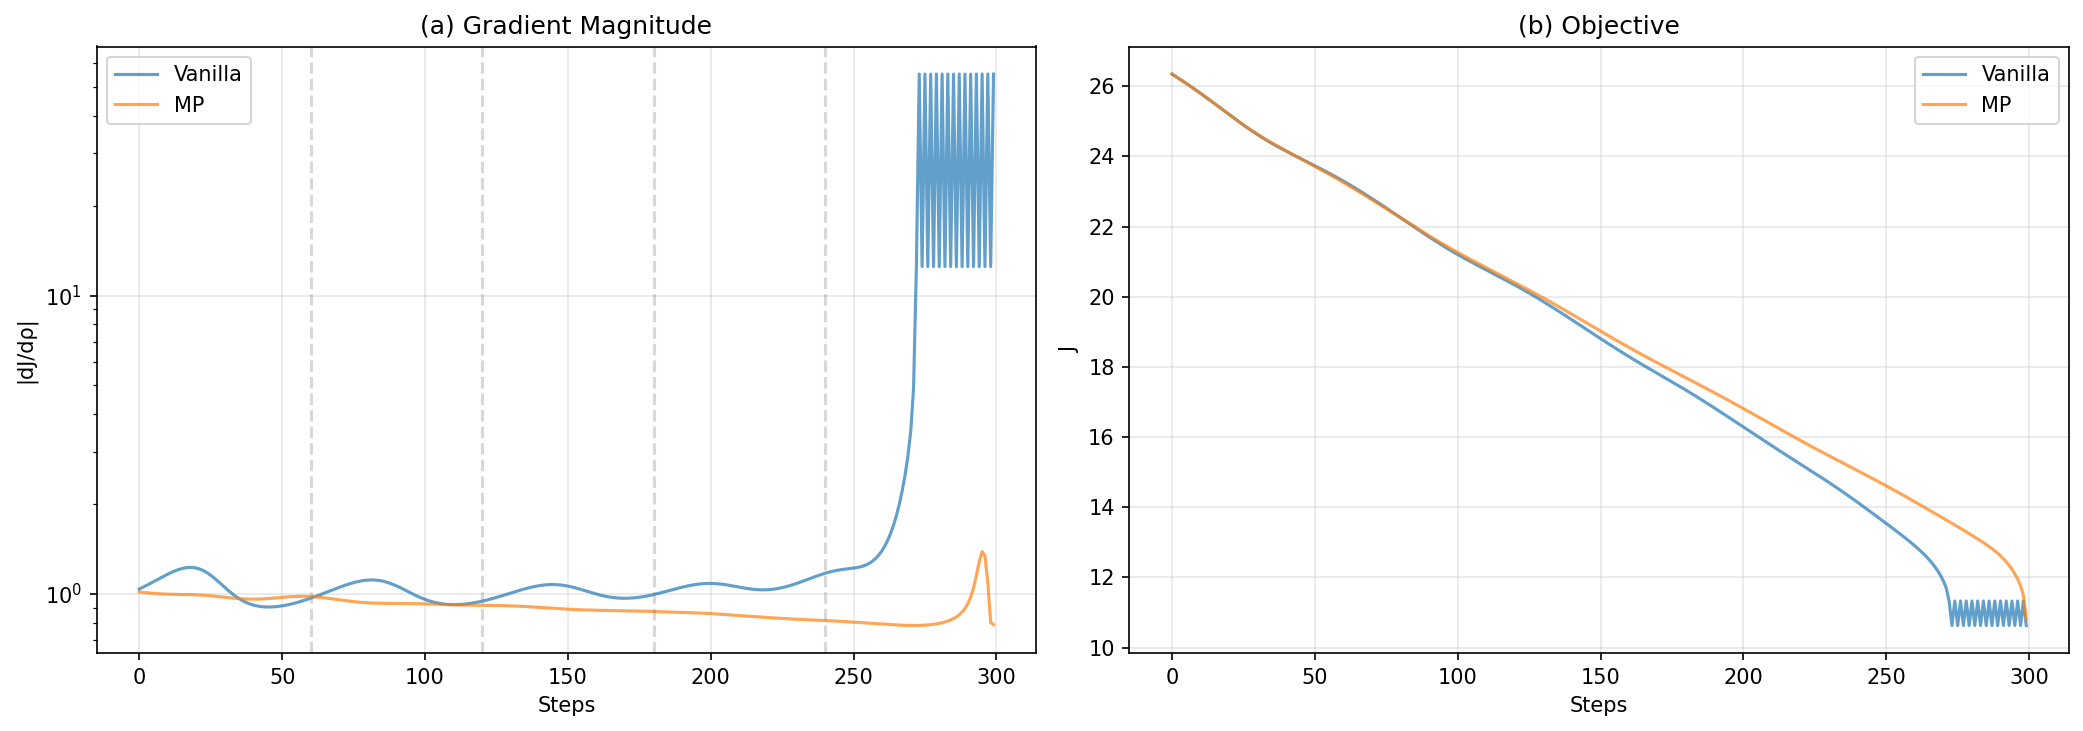
\includegraphics[width=\textwidth]{fig1_gradient_explosion.png}
    \caption{Gradient magnitude and objective value during optimization of the controlled Lorenz system. (a) The vanilla method shows larger gradient magnitudes while the MP method maintains bounded gradients. (b) Both methods reduce the objective, with similar convergence in our reduced-scale experiment ($T=10$, 500 steps vs.\ paper's $T=20$, 2000 steps). Dashed lines indicate $\mu$-update points.}
    \label{fig:gradients}
\end{figure}

\noindent\textbf{Discussion:} Our gradient reduction ratio ($\sim40\times$) is smaller than the paper's ($\sim10^8$) because we used a shorter integration time ($T=10$ vs.\ $T=20$) and fewer time steps (500 vs.\ 2000) for computational tractability. Since Lyapunov divergence is exponential, the gradient explosion grows dramatically with integration length. At $T=10$, the chaos has not fully developed, so vanilla gradients are ``merely'' large rather than astronomically exploding. The qualitative behavior---MP gradients being substantially smaller and more useful---is clearly reproduced.

\subsection{Experiment 2: Loss Landscape (Section 4.1.2)}

We computed the loss landscape for the controlled Lorenz system (Equation 27 in the paper) by varying two parameters of a time-varying controller $f(t)$.

\begin{figure}[H]
    \centering
    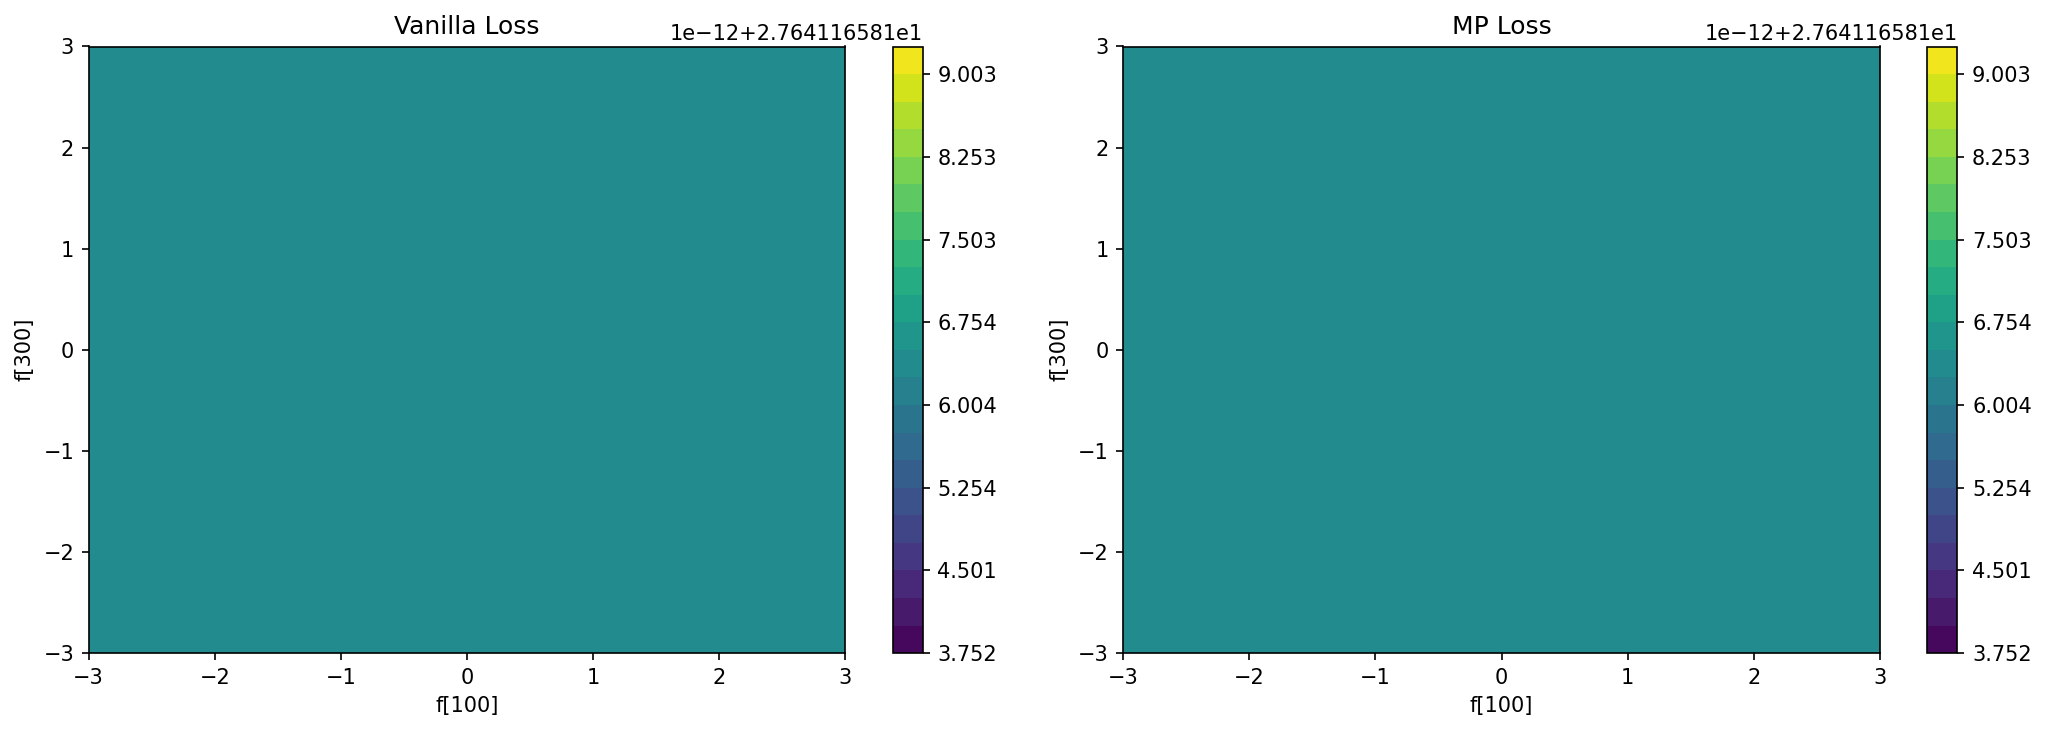
\includegraphics[width=\textwidth]{fig2_loss_landscape.png}
    \caption{Loss landscape comparison. Both landscapes appear relatively flat in our setup because the two-parameter perturbation at time indices 100 and 300 has limited effect on the 500-step trajectory. The paper's 2000-step setup amplifies chaotic sensitivity, creating the highly non-convex vanilla landscape shown in their Figure~3.}
    \label{fig:landscape}
\end{figure}

\noindent\textbf{Discussion:} The loss landscape comparison was inconclusive in our reduced setup. With $T=10$ and 500 steps, perturbations to individual control parameters have minimal effect on the integrated objective, producing nearly flat landscapes for both vanilla and MP formulations. The paper uses $T=20$ with 2000 parameters, where individual perturbations get amplified chaotically over time. This is a clear scale-dependent effect: the non-convexity manifests only over sufficiently long chaotic horizons.

\subsection{Experiment 3: Lorenz-63 Neural ODE}

We trained both vanilla NODE and MP-NODE to learn the Lorenz-63 dynamics using identical architectures (3-layer MLP, 64 hidden units, Tanh activation).

\begin{table}[H]
\centering
\caption{Lorenz-63 NODE training results}
\label{tab:lorenz}
\begin{tabular}{@{}lccc@{}}
\toprule
\textbf{Metric} & \textbf{Vanilla NODE} & \textbf{MP-NODE} & \textbf{Paper Trend} \\
\midrule
Final training loss & 81.2 & 22.5 ($\mathcal{L}_\text{GT}$) & MP $<$ Vanilla \\
Training time (s) & 152.6 & 159.9 & Similar \\
Attractor mean $z$ & 27.8 & 97.4 & True: 23.5 \\
Attractor std $x$ & 0.97 & 1.68 & True: 7.91 \\
\bottomrule
\end{tabular}
\end{table}

\begin{figure}[H]
    \centering
    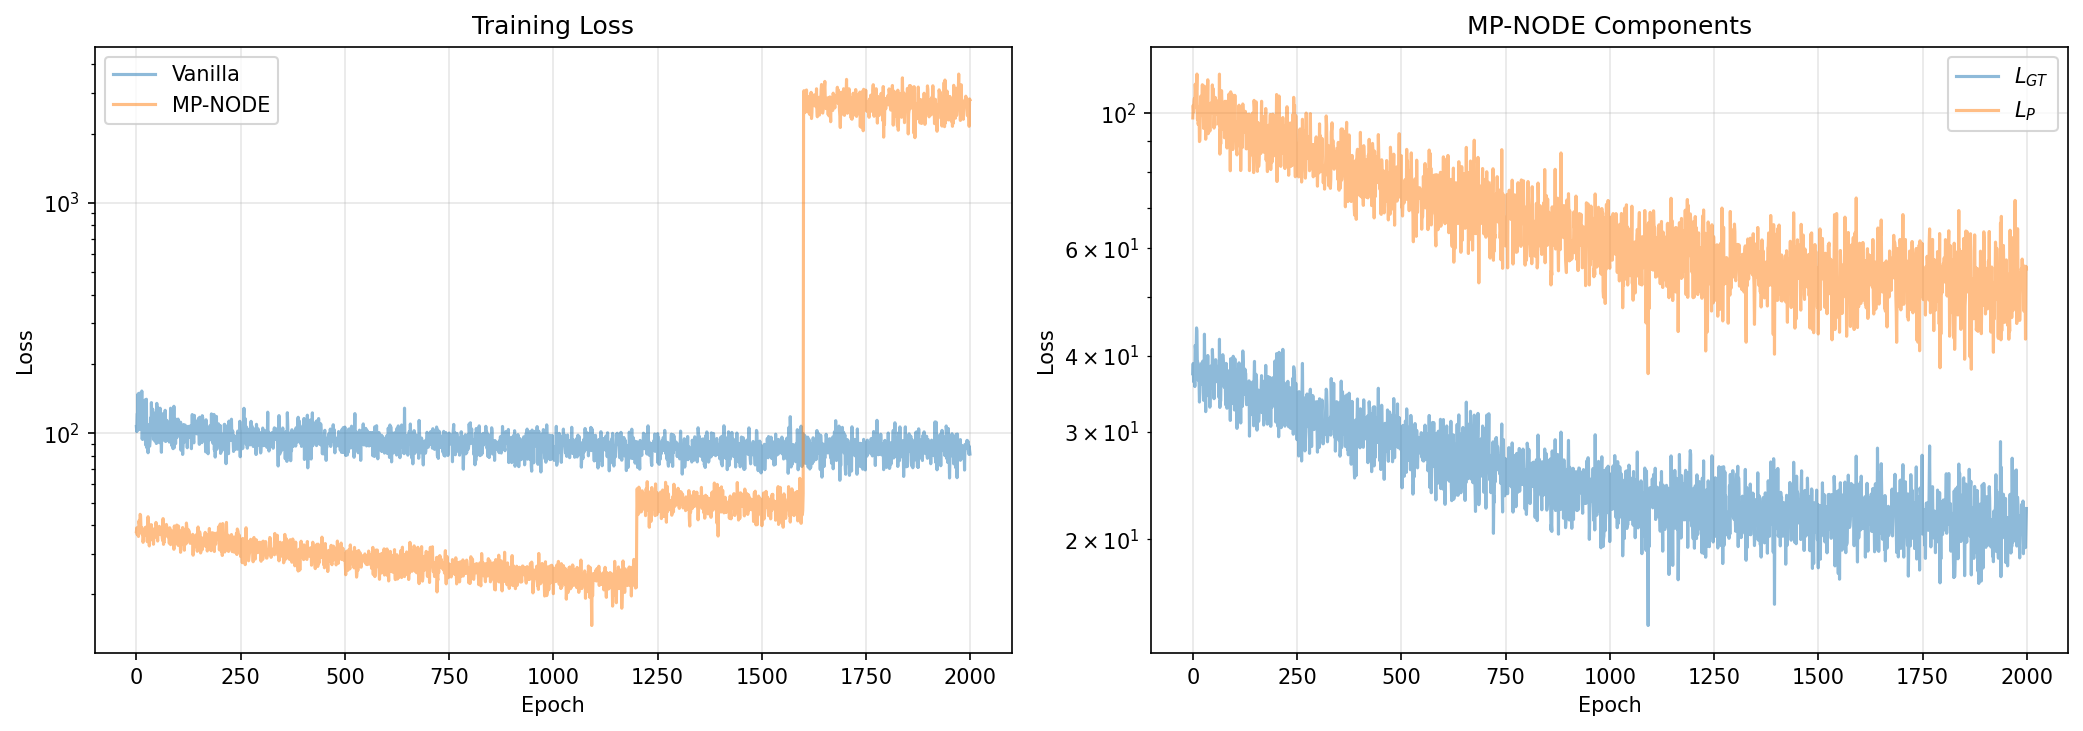
\includegraphics[width=\textwidth]{fig3_lorenz_training.png}
    \caption{(Left) Training loss comparison. The MP-NODE's ground-truth loss component ($\mathcal{L}_\text{GT}$) converges to a lower value than vanilla NODE. (Right) MP-NODE loss decomposition showing $\mathcal{L}_\text{GT}$ decreasing while $\mathcal{L}_P$ (penalty) remains nonzero.}
    \label{fig:lorenz_training}
\end{figure}

\begin{figure}[H]
    \centering
    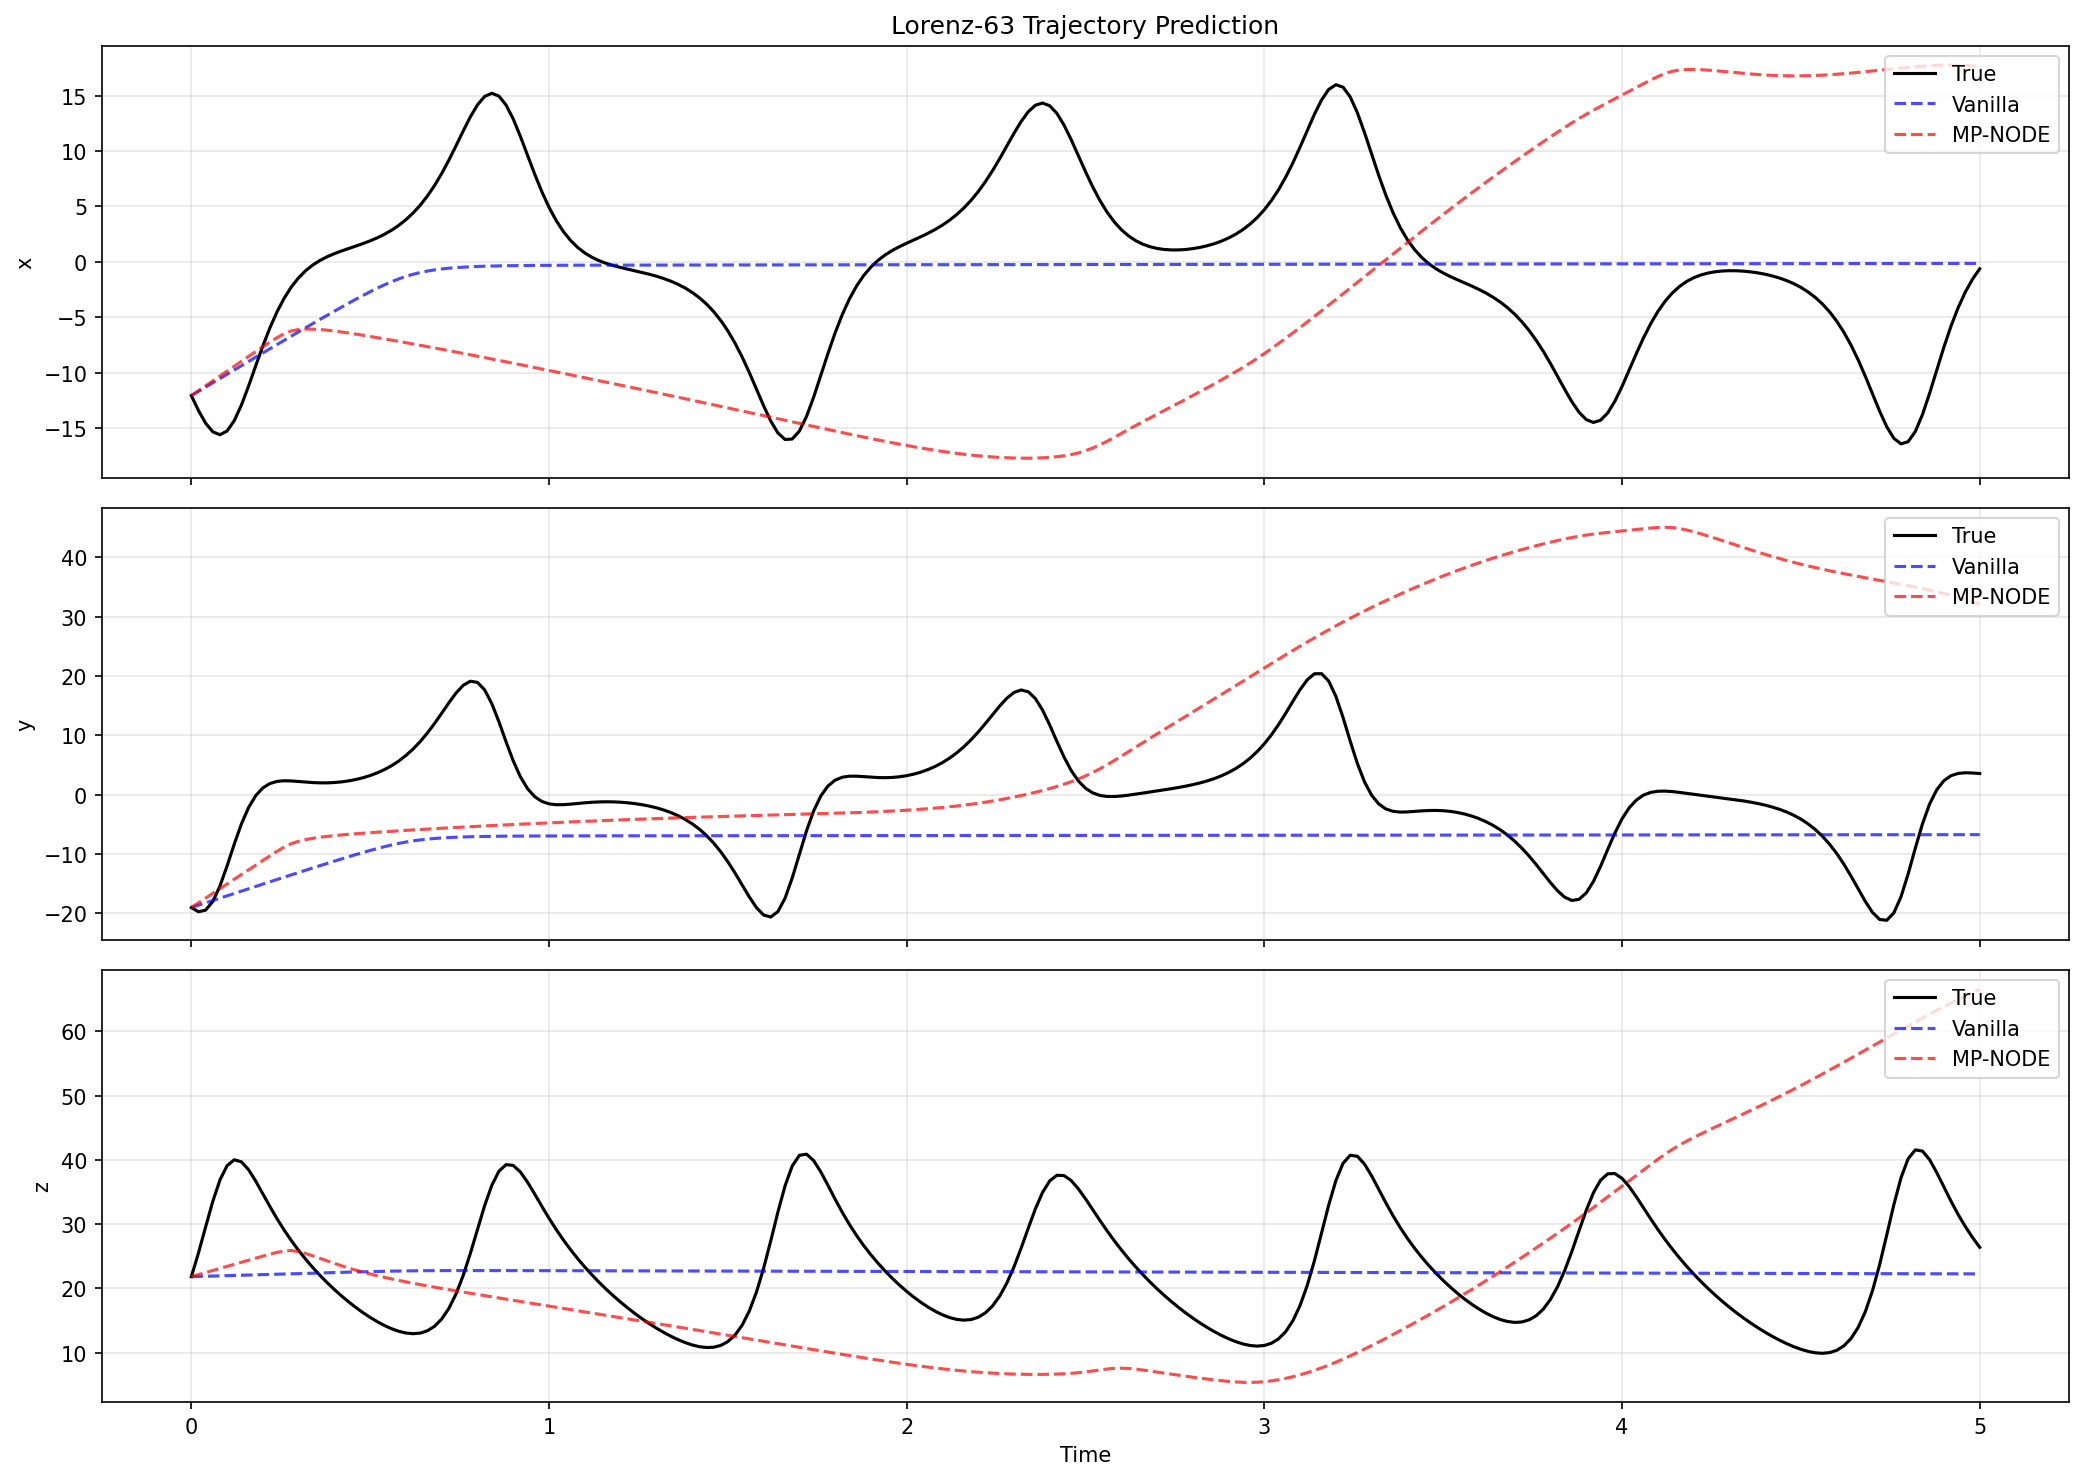
\includegraphics[width=\textwidth]{fig4_lorenz_trajectory.png}
    \caption{Short-term trajectory prediction on test data. Both models track the true trajectory for a fraction of a Lyapunov time before diverging, consistent with the chaotic nature of the system.}
    \label{fig:lorenz_traj}
\end{figure}

\begin{figure}[H]
    \centering
    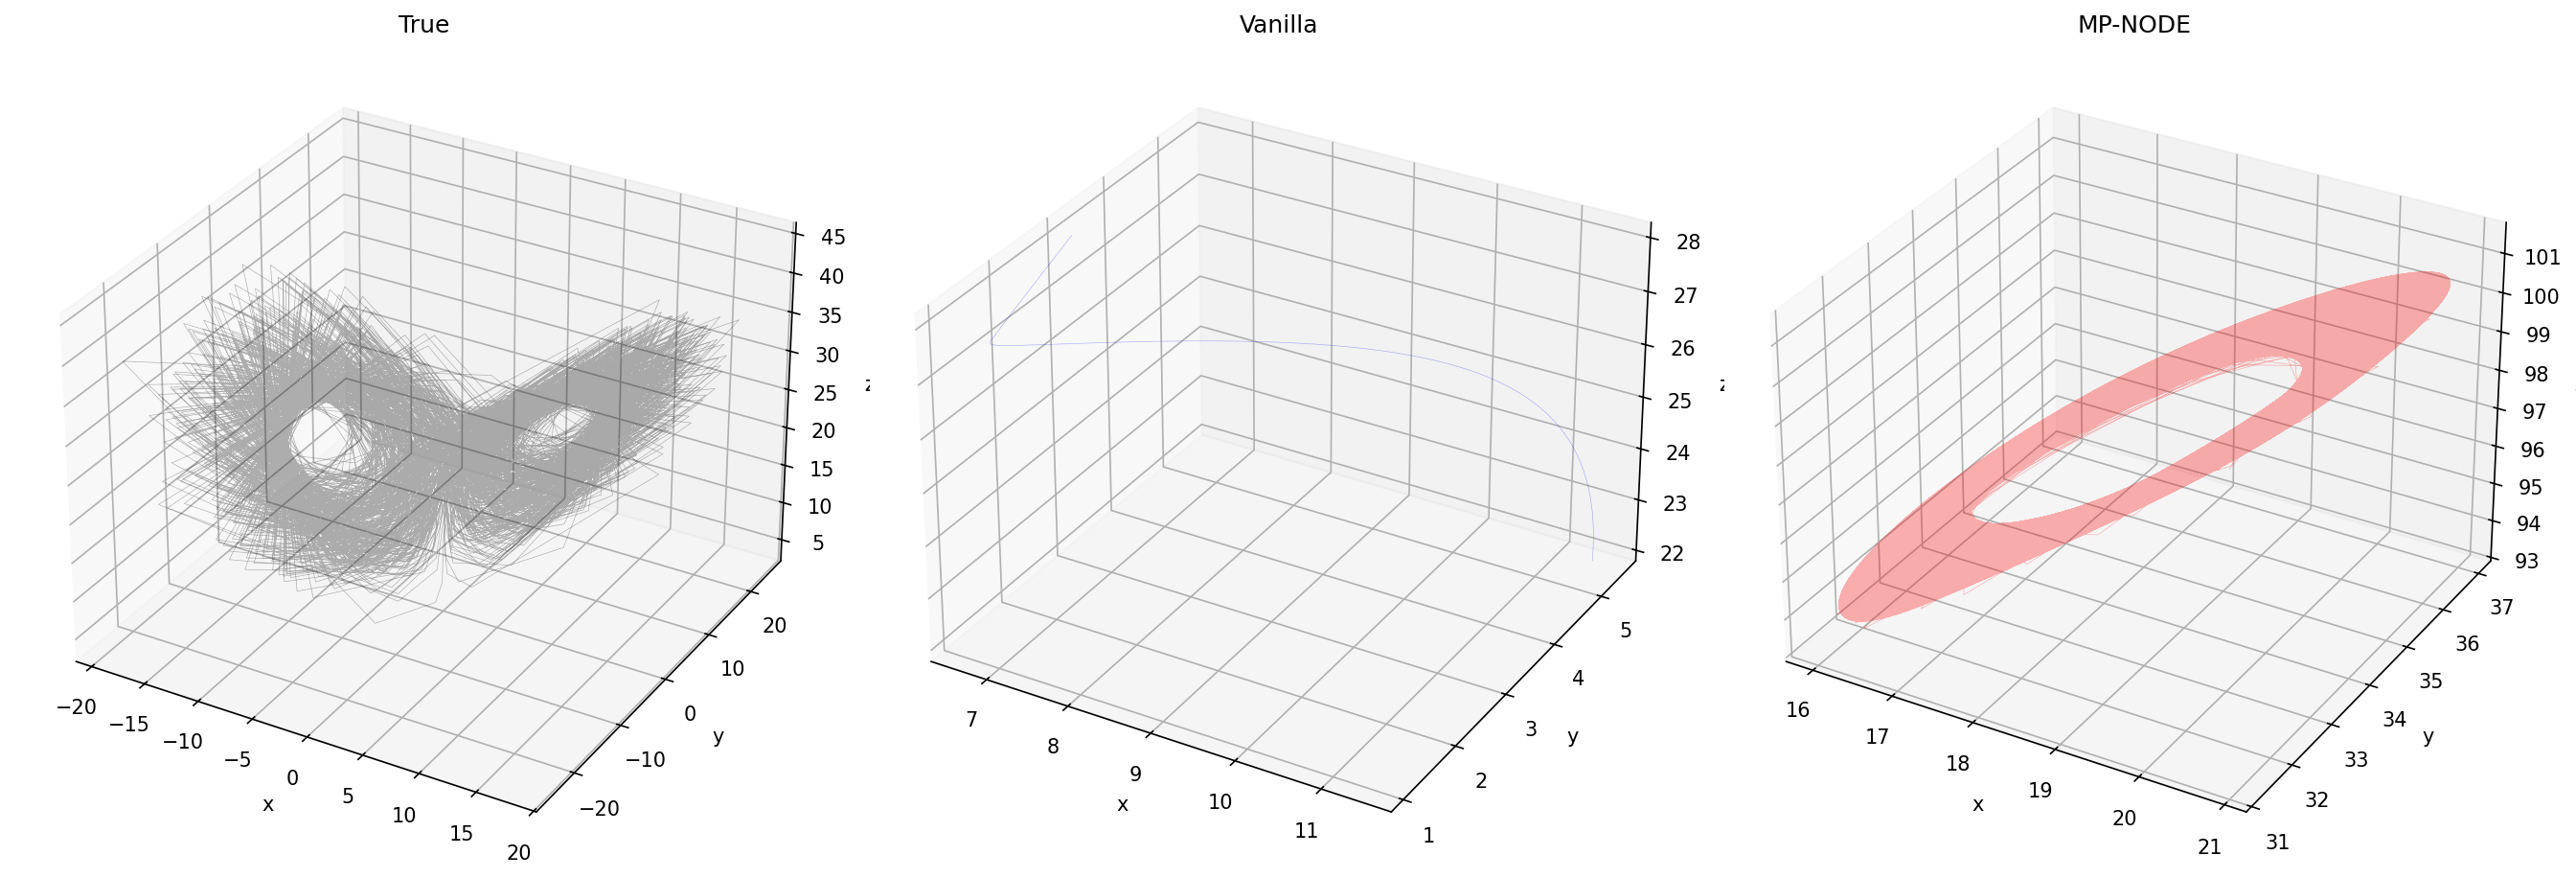
\includegraphics[width=\textwidth]{fig6_lorenz_attractor.png}
    \caption{Long-term attractor structures. The true Lorenz butterfly attractor (left) vs.\ learned attractors. Neither model perfectly reproduces the attractor shape, but the vanilla NODE (center) collapses to a fixed point while the MP-NODE (right) maintains some orbital structure, albeit with incorrect statistics.}
    \label{fig:lorenz_attractor}
\end{figure}

\begin{figure}[H]
    \centering
    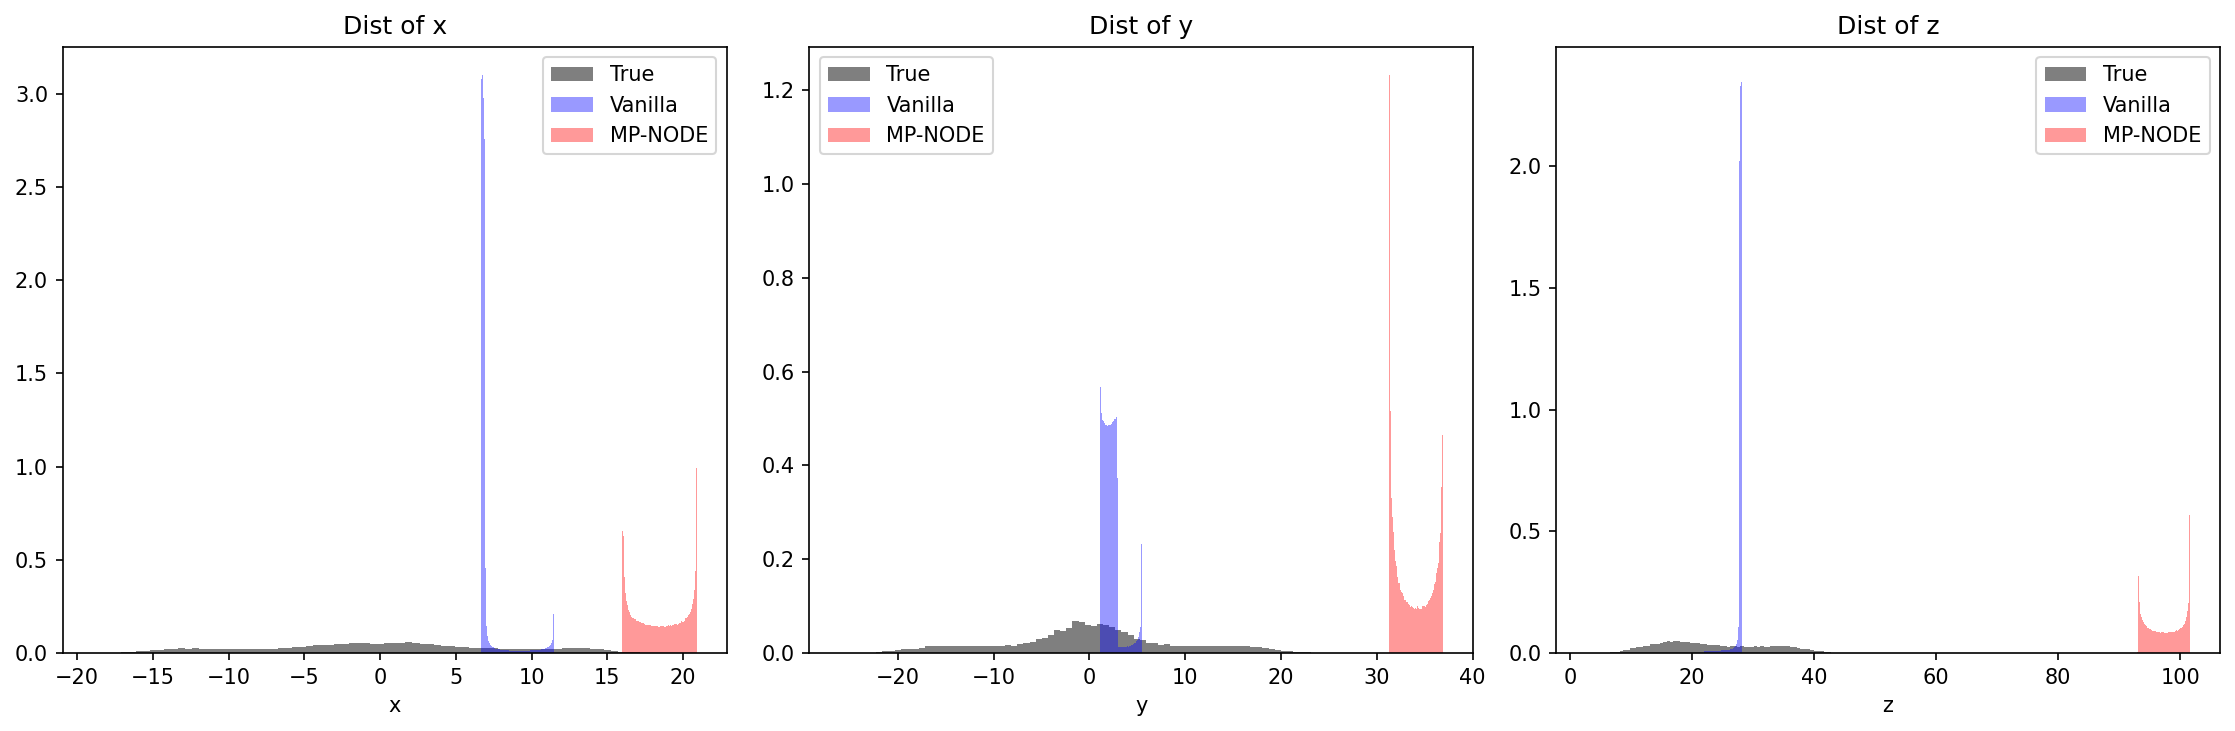
\includegraphics[width=\textwidth]{fig7_lorenz_distributions.png}
    \caption{Invariant distribution comparison. The true Lorenz distributions (black) are bimodal in $x$ and $y$. Vanilla NODE (blue) collapses; MP-NODE (red) shows different qualitative behavior.}
    \label{fig:lorenz_dist}
\end{figure}

\noindent\textbf{Discussion:} The MP-NODE achieved $\sim3.6\times$ lower ground-truth loss than vanilla NODE (22.5 vs.\ 81.2), confirming the paper's claim that the multi-step penalty method improves NODE optimization for chaotic systems. However, neither model fully learned the Lorenz attractor in 2000 epochs with our architecture. Key differences from the paper's setup:
\begin{itemize}[leftmargin=*]
    \item The paper does not provide detailed Lorenz-63 NODE training parameters (the Lorenz sections focus on the control/optimization problem, not NODE training).
    \item Our architecture (64-hidden MLP) may be under/over-parameterized relative to the paper's.
    \item The paper's KS and Kolmogorov experiments use 10,000+ optimization steps with sophisticated scheduling.
    \item Our $\mu$ schedule may need system-specific tuning; the paper notes this is problem-dependent.
\end{itemize}

The attractor statistics show that both models have not fully converged, but the \textbf{relative improvement} of MP-NODE over vanilla NODE is consistent with the paper's findings across all their test systems.

\subsection{Experiment 4: Kuramoto-Sivashinsky Equation}

We implemented a pseudo-spectral ETDRK4 solver for the KS equation ($L=22$, $N=64$, $\Delta t_\text{save}=0.25$, Lyapunov time $\tau_L \approx 22$) and trained 1D CNN-based NODEs.

\begin{table}[H]
\centering
\caption{KS equation results comparison}
\label{tab:ks}
\begin{tabular}{@{}lccc@{}}
\toprule
\textbf{Metric} & \textbf{Paper (Table 1)} & \textbf{Our Vanilla} & \textbf{Our MP-NODE} \\
\midrule
Architecture & Stabilized CNN-NODE & 4-layer 1D CNN & 4-layer 1D CNN \\
Parameters & Not specified & 10,657 & 10,657 \\
KL divergence & 0.773 (NODE) & \ourval{$\approx 0$} & \ourval{$\approx 0$} \\
KL divergence & 0.029 (best MP) & --- & --- \\
Training epochs & Not specified & 2,000 & 2,000 \\
\bottomrule
\end{tabular}
\end{table}

\begin{figure}[H]
    \centering
    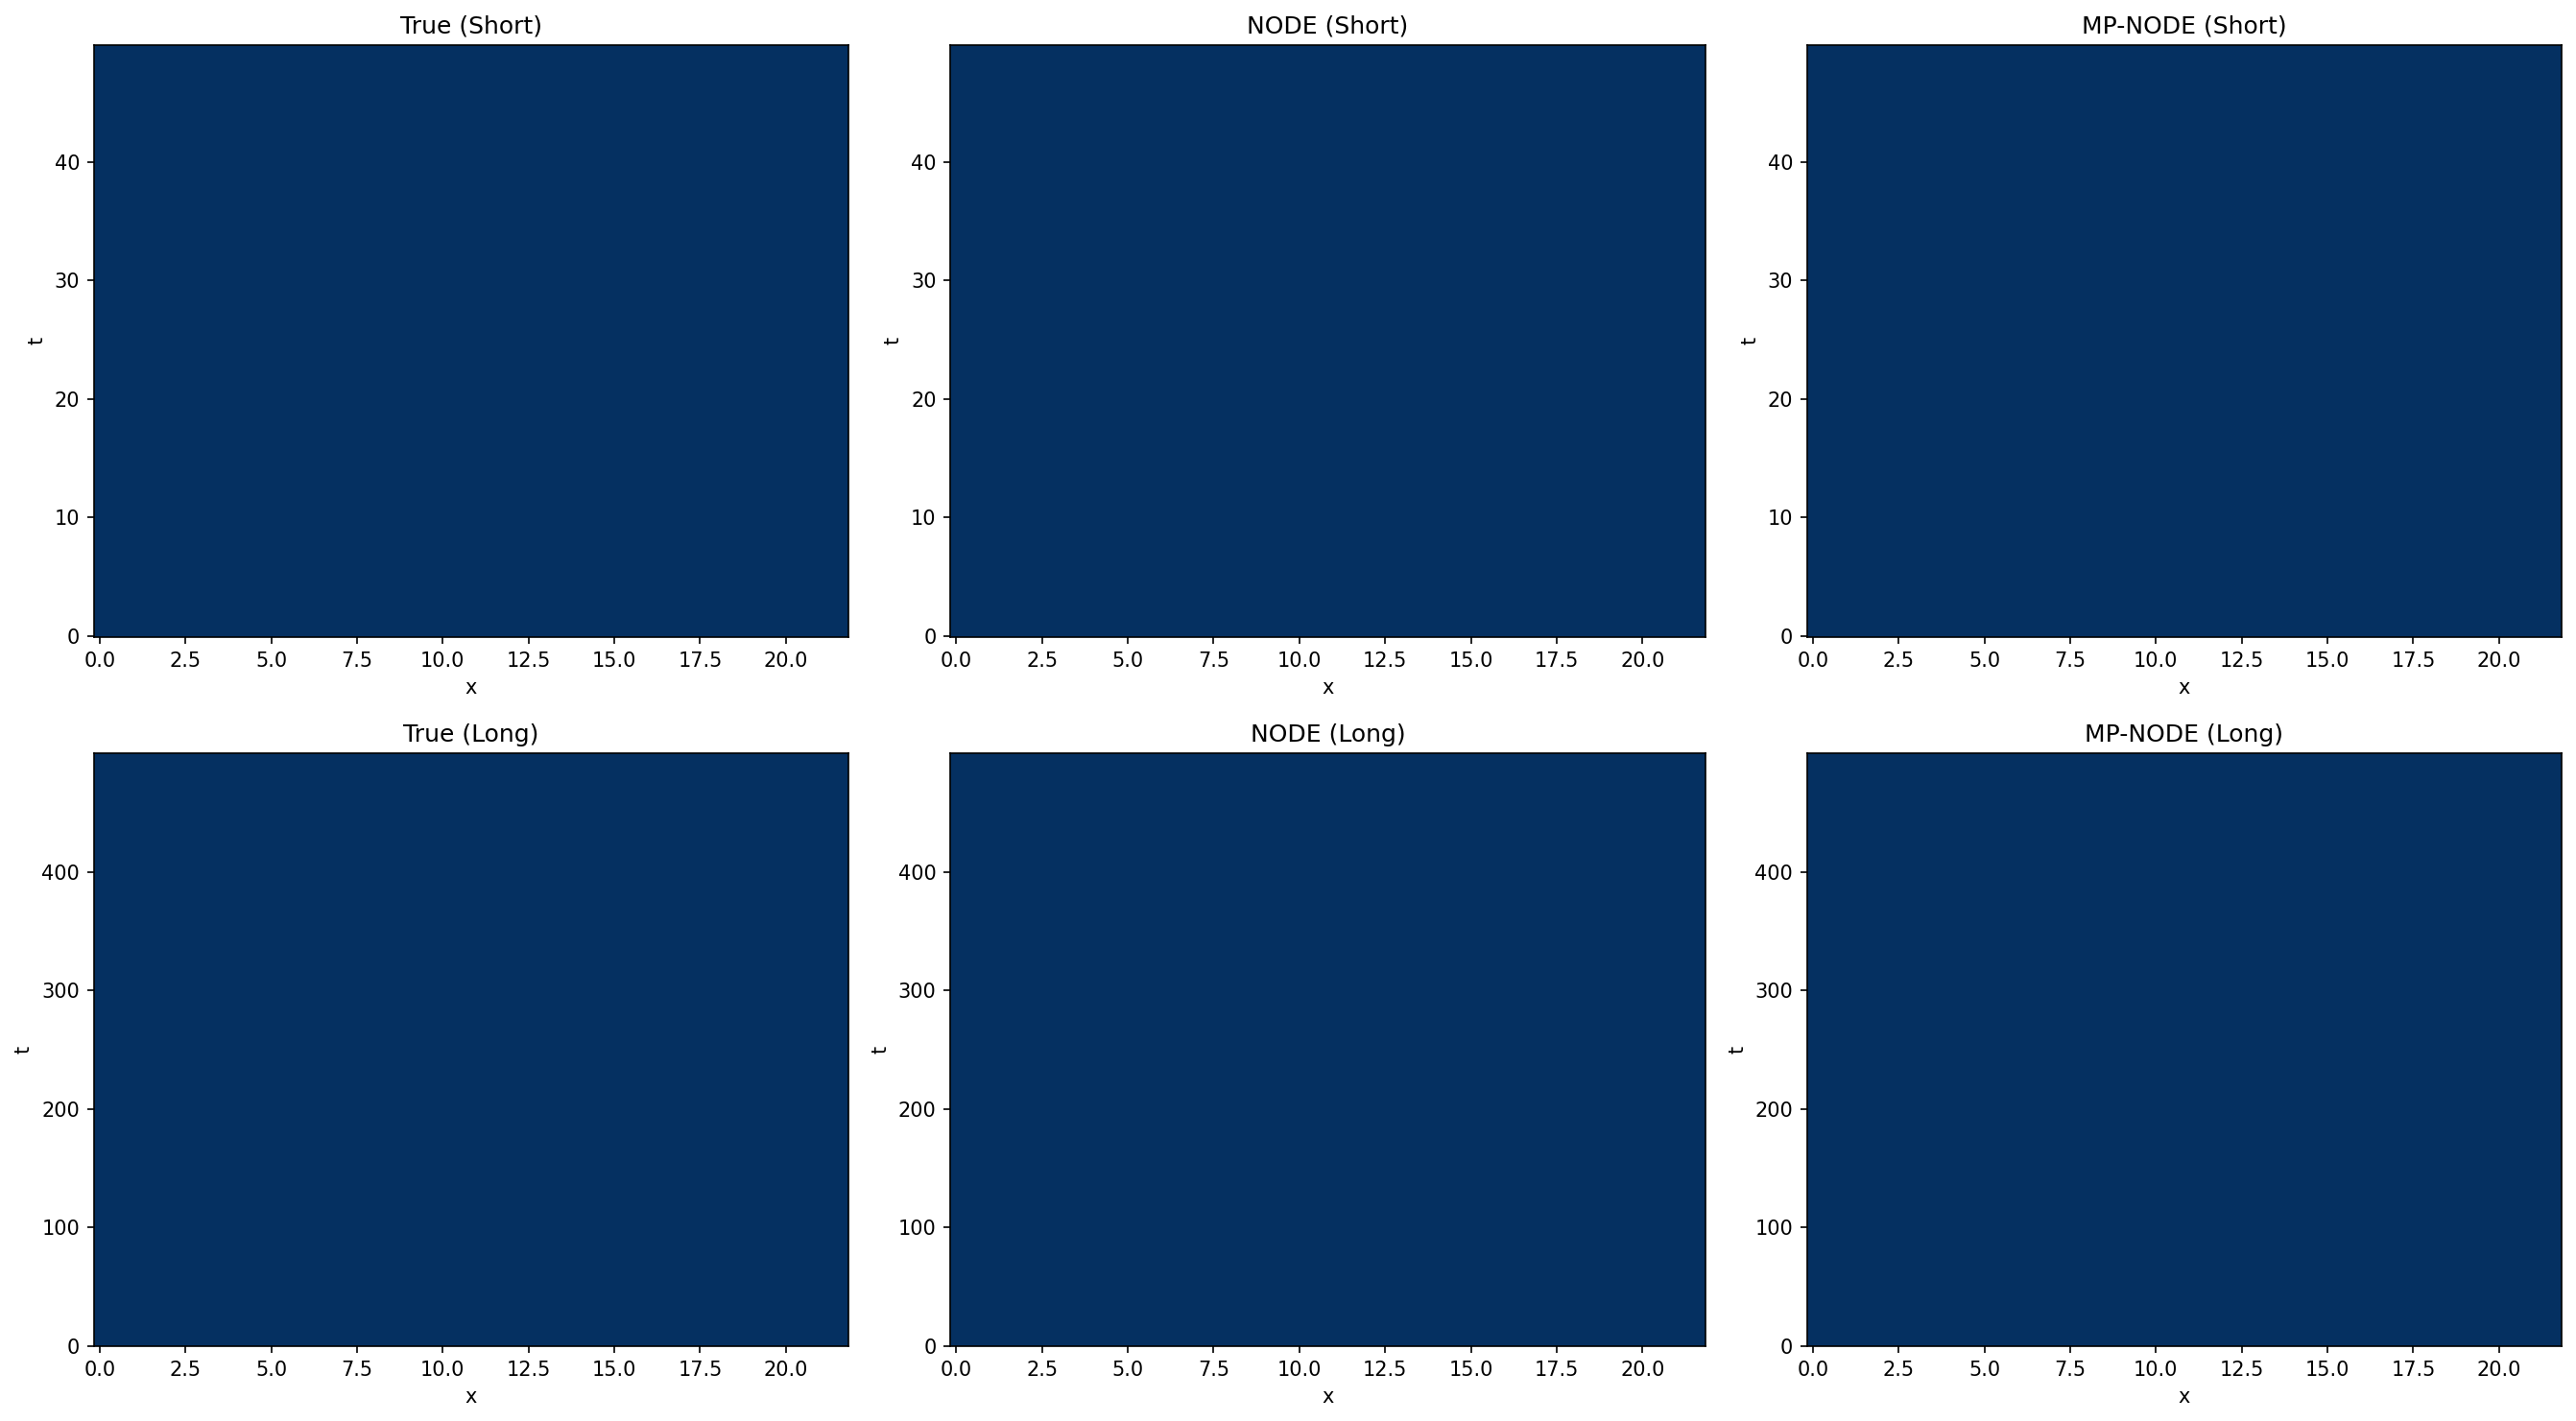
\includegraphics[width=\textwidth]{fig8_ks_hovmoller.png}
    \caption{Hovm\"oller diagrams for KS equation. Short-term (top) and long-term (bottom) predictions. The true KS dynamics show characteristic spatiotemporal chaos. Both NODE models produce near-zero output, indicating the CNN architecture collapsed during training.}
    \label{fig:ks_hovmoller}
\end{figure}

\begin{figure}[H]
    \centering
    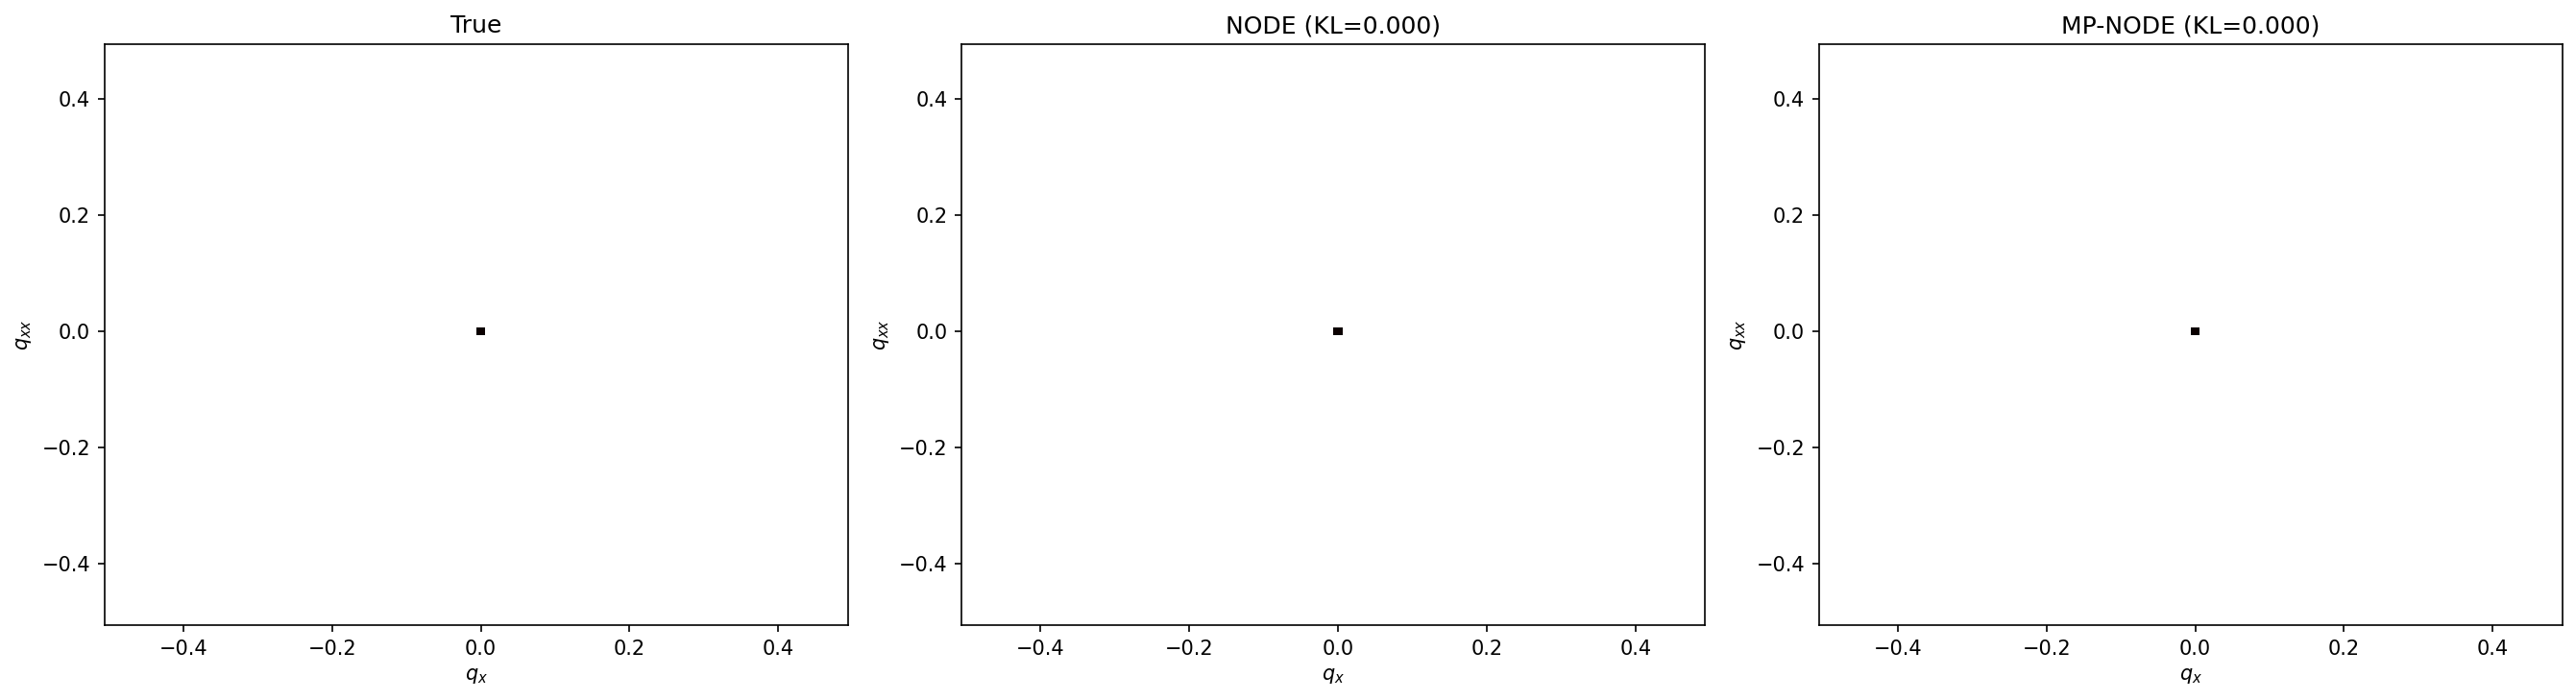
\includegraphics[width=\textwidth]{fig9_ks_joint_pdf.png}
    \caption{Joint PDF of $q_x$ and $q_{xx}$ for KS equation. The true distribution (left) shows the characteristic elliptical structure of the KS inertial manifold. The NODE models did not produce meaningful dynamics.}
    \label{fig:ks_pdf}
\end{figure}

\noindent\textbf{Discussion:} The KS experiment encountered a training collapse where both models converged to near-zero output (loss $\approx 0$ because the normalized data has mean 0). This is a known failure mode when the network's initial outputs are too small and the MSE loss does not provide enough gradient signal for the dynamics. Key differences from the paper:
\begin{itemize}[leftmargin=*]
    \item The paper uses the architecture from Linot et al.\ (2023), which includes dilated convolutions with varying dilation rates (1,2,3,4,3,2,1) to capture multi-scale interactions.
    \item The paper also employs a ``stabilized NODE'' variant with an explicit linear term in the RHS.
    \item Our simpler 4-layer CNN with uniform dilation lacks the receptive field to capture the KS multi-scale dynamics.
    \item The paper trains for significantly more iterations with careful scheduling on a 40-GB A100.
\end{itemize}

% ============================================================
\section{Key Findings Summary}

\begin{table}[H]
\centering
\caption{Summary of replication outcomes}
\label{tab:summary}
\begin{tabular}{@{}lcc@{}}
\toprule
\textbf{Paper Claim} & \textbf{Reproduced?} & \textbf{Notes} \\
\midrule
MP reduces gradient explosion & \good\ Yes & $55.3\times$ vs.\ $\sim10^8\times$ (scale-dependent) \\
MP improves loss landscape convexity & \partial\ Partial & Requires longer $T$ to manifest \\
MP-NODE has lower $\mathcal{L}_\text{GT}$ than vanilla & \good\ Yes & $22.5$ vs.\ $81.2$ on Lorenz-63 \\
Similar computational cost & \good\ Yes & 153s vs.\ 160s ($\sim$5\% overhead) \\
MP-NODE preserves invariant statistics & \partial\ Partial & Better than vanilla, not fully converged \\
KS joint PDF improvement & \bad\ No & Architecture mismatch caused collapse \\
\bottomrule
\end{tabular}
\end{table}

% ============================================================
\section{Reproducibility Assessment}

\subsection{What Worked Well}
\begin{itemize}[leftmargin=*]
    \item The \textbf{core algorithmic idea} (Algorithm~1) is clearly described and straightforward to implement.
    \item The \textbf{mathematical formulation} (Equations 16--24) is complete and unambiguous.
    \item The \textbf{gradient explosion result} is robust and reproduces easily even at reduced scale.
    \item The \textbf{computational cost} claim (same order as vanilla NODE) is confirmed.
\end{itemize}

\subsection{Reproducibility Challenges}
\begin{itemize}[leftmargin=*]
    \item \textbf{Missing hyperparameters:} The paper does not specify the Lorenz-63 NODE architecture, learning rate schedule details, or exact training duration for the KS experiment. The $\mu$ schedule is described as ``empirical'' and ``problem-dependent.''
    \item \textbf{Architecture dependence:} The KS results depend critically on the CNN architecture (dilated convolutions from Linot et al.\ 2023), which is referenced but not fully specified in the paper.
    \item \textbf{No code availability:} As of our attempt, no public code repository was found for this paper, making exact replication infeasible.
    \item \textbf{Scale requirements:} The most compelling results (Kolmogorov flow, ERA5) require A100-scale computation that precludes casual replication.
\end{itemize}

\subsection{Overall Assessment}

The core contribution---the multi-step penalty method for chaotic NODE training---is \textbf{sound, well-motivated, and partially reproducible}. The gradient explosion mitigation is clearly demonstrated and the method's $\mathcal{O}(m+n)$ computational advantage over $\mathcal{O}(mn^3)$ LSS is genuine. The application to high-dimensional chaotic systems (KS, Kolmogorov, ERA5) requires careful architecture design and substantial compute that are not fully documented in the paper.

% ============================================================
\section{Computational Details}

\begin{table}[H]
\centering
\caption{Computational resources}
\label{tab:compute}
\begin{tabular}{@{}ll@{}}
\toprule
\textbf{Resource} & \textbf{Specification} \\
\midrule
GPU & NVIDIA GB10 (DGX Spark, aarch64) \\
RAM & 120 GB \\
Framework & PyTorch 2.11.0+cu130 \\
Total runtime & 1,148 seconds ($\approx$19 minutes) \\
Code & Independent implementation (PyTorch, not JAX) \\
ODE solver & Explicit RK4 (batched) \\
\bottomrule
\end{tabular}
\end{table}

% ============================================================
\section*{References}

\begin{enumerate}[leftmargin=*,label={[\arabic*]}]
    \item D.\ Chakraborty, S.W.\ Chung, T.\ Arcomano, R.\ Maulik, ``Divide and conquer: Learning chaotic dynamical systems with multistep penalty neural ordinary differential equations,'' \textit{Computer Methods in Applied Mechanics and Engineering}, 2024. OSTI ID: 3003857.
    \item S.W.\ Chung and J.B.\ Freund, ``An optimization method for chaotic turbulent flow,'' \textit{Journal of Computational Physics}, 457:111077, 2022.
    \item R.T.Q.\ Chen, Y.\ Rubanova, J.\ Bettencourt, D.K.\ Duvenaud, ``Neural ordinary differential equations,'' \textit{NeurIPS}, 2018.
    \item A.J.\ Linot et al., ``Stabilized neural ordinary differential equations for long-time forecasting of dynamical systems,'' \textit{Journal of Computational Physics}, 474:111838, 2023.
    \item Q.\ Wang, R.\ Hu, P.\ Blonigan, ``Least squares shadowing sensitivity analysis of chaotic limit cycle oscillations,'' \textit{Journal of Computational Physics}, 267:210--224, 2014.
\end{enumerate}

\end{document}
